\documentclass[11pt,a4j]{jarticle}
\usepackage{amsmath,amsthm,amssymb}
\usepackage{type1cm}
\usepackage[dvipdfmx]{graphicx}
\usepackage{float}
\usepackage{subcaption}

\title{包絡線定理の作図プログラム}
\author{田中 雅樹}
\date{2014/06/07}

\begin{document}

\maketitle

\begin{abstract}
本稿は、包絡線および包絡線定理の解説を行った上で、筆者が作成した包絡線の作図プログラム\footnote{使用言語はPythonである}を紹介するものである。

経済学では最適化問題の結果として様々な関数が得られるが、そこにおいて「包絡線」という概念が非常に重要である。
包絡線の重要性の一方で、包絡線の作図は時として非常に煩雑なものとなる。
今回作成した作図プログラムは、適宜設定を変更することで、多様な関数を用いて作図することが可能であり、包絡線に関する様々な場面で有用なプログラムと言える。
\end{abstract}

\section{はじめに}
パラメタを含む関数$f$が与えられたときに、そのパラメタの値を変化させることで$f$のグラフも変化させることができる。
こうして得られた曲線群の共通接線となるような曲線のことを\textbf{包絡線}(envelop)と呼ぶ。

図\ref{fig:envelope}は、関数$y=2tx-t^{2}$に関して、パラメタ$t$を規則的に変化させた時の様子を示している。
このケースでは放物線$y=x^{2}$が包絡線となっており、図からもその様子がはっきりと見て取ることができる。

今回作成した作図プログラムは、このような包絡線を説明する際に必要なグラフを作成することができるプログラムである。
適宜設定を変更することで、$y=2tx-t^{2}$のような簡単な関数形だけでなく、より複雑な関数を用いて作図することも可能であり、包絡線に関する様々な場面で有用なプログラムとなっている。

\begin{figure}
 \centering
 \begin{subfigure}{0.4\columnwidth}
  \centering
  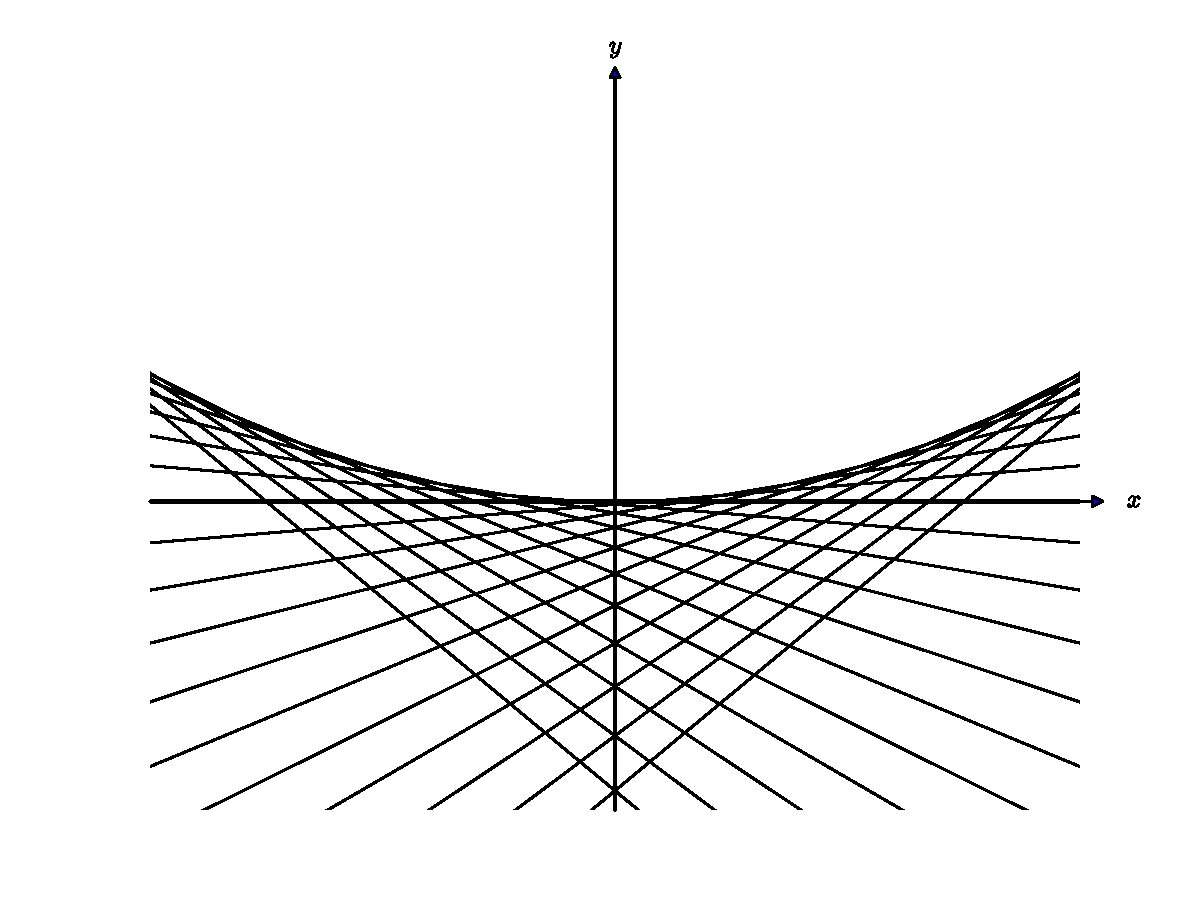
\includegraphics[scale=0.3]{envelope0.pdf}
  \caption{包絡線(粗)}
  \label{fig:envelope0}
 \end{subfigure}
 \begin{subfigure}{0.4\columnwidth}
  \centering
  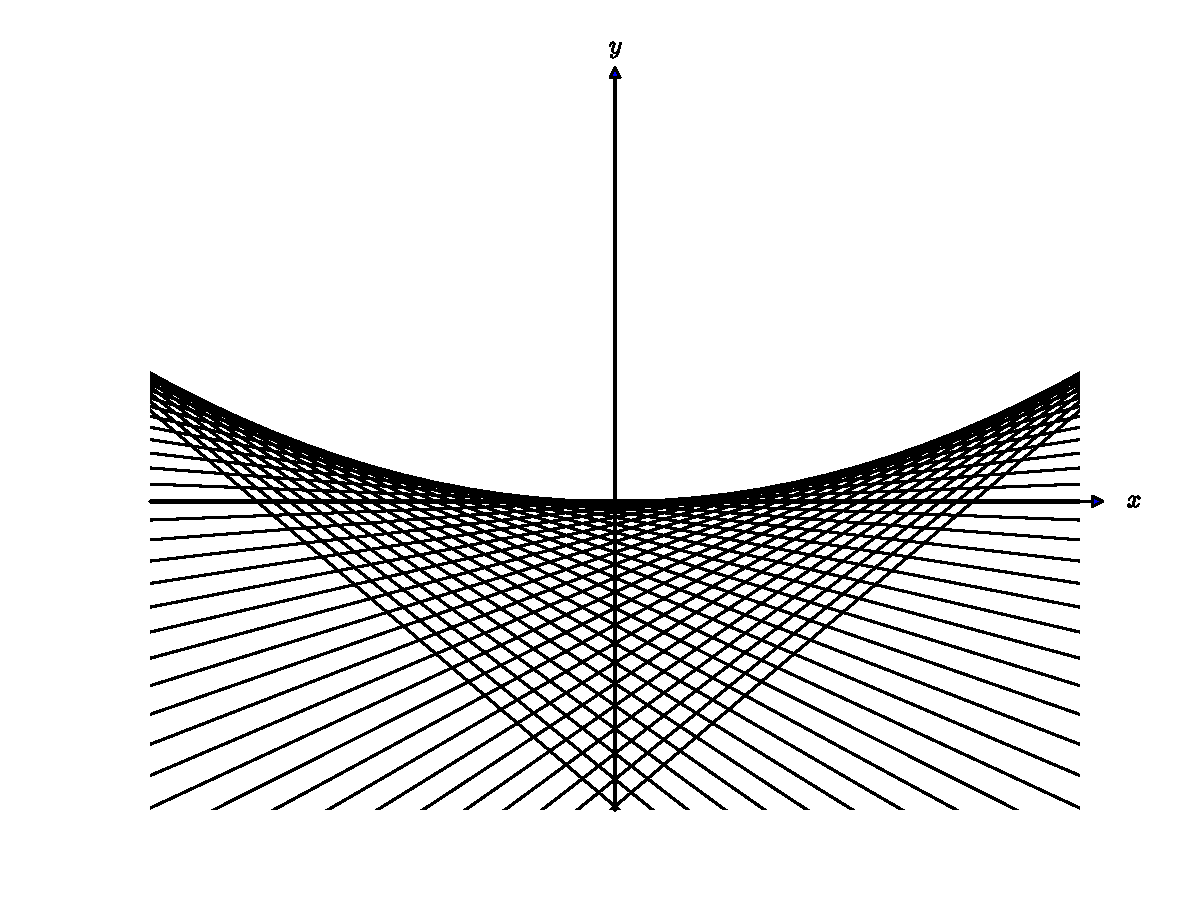
\includegraphics[scale=0.3]{envelope1.pdf}
  \caption{包絡線(密)}
  \label{fig:envelope1}
 \end{subfigure}
 \caption{包絡線の例}
 \label{fig:envelope}
\end{figure}


\section{包絡線定理}
次のような\textbf{最大値関数}(maximum value function)を考える。
\[ v(\alpha)=\max_{x}f(x,\alpha) \]
\[ x\in \mathbb{R}^{n} ,\alpha \in \mathbb{R}^{n}\]
上式右辺の最大化問題の解を$x^{*}(\alpha)$とする。
つまり、
\[ v(\alpha)=\max_{x}f(x^{*}(\alpha),\alpha) \]
となっている。
ここで、最大化の一階条件(First-Order Condition; FOC)より、
\[ \frac{\partial f}{\partial x_{i}}(x^{*}(\alpha),\alpha) = 0 \]
が成り立っている。
すると、合成関数の微分の公式を使うと、
\begin{eqnarray*}
 \frac{\partial v}{\partial \alpha_{j}}&=&\frac{\partial}{\partial \alpha_{j}}f(x^{*}(\alpha),\alpha)\\
 &=&\sum^n_{i=1}\frac{\partial f}{\partial x^{*}_{i}}(x^{*}(\alpha),\alpha)\frac{\partial x^{*}_{i}}{\partial \alpha_{j}}(\alpha)+\frac{\partial f}{\partial \alpha_{j}}(x^{*}(\alpha),\alpha)\\
 &=&\frac{\partial f}{\partial \alpha_{j}}(x^{*}(\alpha),\alpha)
\end{eqnarray*}
となる(上記の計算において、シグマ内にFOCが使われていることに注意したい)。

ここで$\alpha=\Bar{\alpha}$と固定して、
\[ \Bar{x} = x^{*}(\Bar{\alpha}) \]
とする。$v$は最大値関数であったので、
\begin{eqnarray*}
 v(\Bar{\alpha}) &=& f(\Bar{x},\Bar{\alpha})\\
 v(\alpha) &\geq& f(\Bar{x},\alpha) \quad \forall\alpha
\end{eqnarray*}
が成り立つ。
これは$\alpha$を任意の$\Bar{\alpha}$に固定して成り立つので、最大値関数$v$が目的関数$f$の包絡線になっていることを意味している。


\section{Pythonプログラム}
ここからは、図\ref{fig:envelope}のところで触れた「包絡線作図プログラム」を紹介することとしたい。
まずはプログラムの全容について記しておく。
\subsection{プログラムの全容}
\begin{quote}
\begin{verbatim}
# -*- coding: utf-8 -*-
from mpl_toolkits.axes_grid.axislines import SubplotZero
from matplotlib.transforms import BlendedGenericTransform
import matplotlib.pyplot as plt
import numpy

z = 25
#グラフを何本引くかを設定します
#y=0があるので、偶数を入力すると左右対称になりません。

u = 1 #グラフ間隔の広さ

x = numpy.linspace(-10, 10, 2) #xの範囲を指定します。

ymin = -240 #グラフ縦方向の下限
ymax = 320 #グラフ縦方向の上限
#この2つはzと連動して適当に決まるようにしたい。

num = 1 
#保存するグラフデータのファイル名につける番号を入力します。
#保存したくない場合はNoneを書きます。

def f(x, t):
    return 2 * t * x - t**2
#包絡線の元となる関数を設定します


fig = plt.figure(1)
ax = SubplotZero(fig, 111)
fig.add_subplot(ax)

ax.axhline(linewidth=1.7, color="black")
ax.axvline(linewidth=1.7, color="black")

plt.xticks([])
plt.yticks([])
plt.ylim([ymin, ymax])

ax.text(0, 1.05, '$y$', transform=BlendedGenericTransform(ax.transData,
 ax.transAxes), ha='center')
ax.text(1.05, 0, '$x$', transform=BlendedGenericTransform(ax.transAxes,
 ax.transData), va='center')

for direction in ["xzero", "yzero"]:
    ax.axis[direction].set_axisline_style("-|>")
    ax.axis[direction].set_visible(True)

for direction in ["left", "right", "bottom", "top"]:
    ax.axis[direction].set_visible(False)

        
for a in range(-z/2 + 1, z/2 + 1):
    y = f(x, t = u * a)
    ax.plot(x, y, linewidth=1, color="black")

if num != None:
    plt.savefig('envelope' + str(num) + '.png')
    plt.savefig('envelope' + str(num) + '.pdf')

plt.show()
\end{verbatim}
\end{quote}
\subsection{プログラムの解説}
このプログラムにおいては、作図するグラフを変えるときに変更すべき箇所をプログラムの冒頭にまとめてある\footnote{具体的には、「$z=$」から「def $f(x,t)$」部までである}。

まずは作図する目的関数$f(x,t)$\footnote{\S1では$y=2tx-t^{2}$、\S2では関数$f$に相当する}を、def $f(x,t):$の次の行で定義する。
このとき$t$がパラメタであり、このプログラムは$t$を指定した範囲で変化させてグラフを描くことに注意すること。

目的関数が定義できた後は、$z$と$u$に数字を設定する。
$z$は「目的関数のグラフを何本引くか」を表す数字であり、数字を大きくすればするほど多くの曲線が引かれる。
$u$は「パラメタをどれぐらいの間隔で動かすか」を表す数字であり、数字を大きくすればするほど曲線の間隔が広くなり、数字を小さくすればするほど曲線の間隔が狭くなる。
図\ref{fig:envelope}では、(a)は$z=25$、$u=1$で作成したグラフであり、$t$を「$-12$から$+12$まで1ごとに」変化させている。
一方、(b)は$z=35$、$u=0.8$で作成したグラフであり、$t$を「$-13.6$から$+13.6$まで0.8ごとに」変化させている。

続いて設定するのは、$x$と$y$の範囲である。
$x$については、numpy.linspace(-10, 10, 2)の括弧内の1番目と2番目の要素によって下限と上限とが設定されているため、
ここを変化させることで設定することができる
\footnote{3番目の要素は、「設定された$x$の範囲内でいくつの点を発生させるか」であるから、直線を考えるのであれば2でよい。なお曲線を考える場合は、適宜増やす必要がある。}。$y$については、yminとymaxに適当な値を設定することで、必要な範囲のグラフを表示させることができる。

最後にnumという変数を説明する。
これは、グラフの保存に関する変数である。
作成された画像は、自動的にPNG形式とPDF形式で保存されるようになっているが、その際につけられるファイル名が「envelop X .png」(Xはnumの値)となる。
なお、numにNoneを割り当てることで、グラフを保存しないようにすることも可能である。


\end{document}
